\subsubsection{\Optimizing MSVC 2010}

\lstinputlisting[caption=\Optimizing MSVC 2010]{patterns/12_FPU/3_comparison/x86/MSVC_Ox/MSVC.asm.\LANG}

\index{x86!\Instructions!FCOM}
\RU{\FCOM отличается от \FCOMP тем, что просто сравнивает значения и оставляет стек в том же состоянии. 
В отличие от предыдущего примера, операнды здесь в обратном порядке. 
Поэтому и результат сравнения в \CThreeBits будет отличаться:}
\EN{\FCOM differs from \FCOMP in the sense that it just compares the values and doesn't change the FPU stack. 
Unlike the previous example, here the operands are in reverse order, 
which is why the result of the comparison in \CThreeBits is different:}

\begin{itemize}
\item
\RU{Если $a>b$, то биты \CThreeBits должны быть выставлены так:}
\EN{If $a>b$ in our example, then \CThreeBits bits are to be set as:} 0, 0, 0.
\item
\RU{Если $b>a$, то биты будут выставлены так:}\EN{If $b>a$, then the bits are:} 0, 0, 1.
\item
\RU{Если $a=b$, то биты будут выставлены так:}\EN{If $a=b$, then the bits are:} 1, 0, 0.
\end{itemize}
% TODO: table?

\RU{Инструкция \TT{test ah, 65} как бы оставляет только два бита~--- \Cthree и \Czero. 
Они оба будут нулями, если $a>b$: в таком случае переход \JNE не сработает. 
\index{ARM!\Instructions!FSTP}
Далее имеется инструкция \TT{FSTP ST(1)}~--- эта инструкция копирует 
значение \ST{0} в указанный операнд и выдергивает одно значение из стека. В данном случае, 
она копирует \ST{0} 
(где сейчас лежит~\TT{\_a})~в~\ST{1}. 
После этого на вершине стека два раза лежит~\TT{\_a}. Затем одно значение выдергивается. 
После этого в \ST{0} остается~\TT{\_a} и функция завершается.}
\EN{The \TT{test ah, 65} instruction leaves just two bits~---\Cthree and \Czero. 
Both will be zero if $a>b$: in that case the \JNE jump will not be triggered. 
Then \TT{FSTP ST(1)} follows~---this instruction copies the value from \ST{0} to the operand and 
pops one value from the FPU stack.
In other words, the instruction copies \ST{0} (where the value of \TT{\_a} is now) into \ST{1}.
After that, two copies of {\_a} are at the top of the stack. 
Then, one value is popped.
After that, \ST{0} contains {\_a} and the function is finishes.}

\RU{Условный переход \JNE сработает в двух других случаях: если $b>a$ или $a=b$. 
\ST{0} скопируется в \ST{0} (как бы холостая операция). 
Затем одно значение из стека вылетит и на вершине стека останется то, что 
до этого лежало в \ST{1} (то~есть~\TT{\_b}). И функция завершится. 
Эта инструкция используется здесь видимо потому что в FPU 
нет другой инструкции, которая просто выдергивает 
значение из стека и выбрасывает его.}
\EN{The conditional jump \JNE is triggering in two cases: if $b>a$ or $a=b$. 
\ST{0} is copied into \ST{0}, it is just like an idle (\ac{NOP}) operation, then one value 
is popped from the stack and the top of the stack (\ST{0}) is contain what was in \ST{1} before 
(that is {\_b}). 
Then the function finishes. 
The reason this instruction is used here probably is because the \ac{FPU} 
has no other instruction to pop a value from the stack and discard it.}

\ifdefined\IncludeOlly
\clearpage
\myparagraph{\RU{Первый пример с \olly: a=1,2 и и=3,4}\EN{First \olly example: a=1.2 and b=3.4}}
\myindex{\olly}

\RU{Обе}\EN{Both} \FLD \RU{отработали}\EN{are executed}:

\begin{figure}[H]
\centering
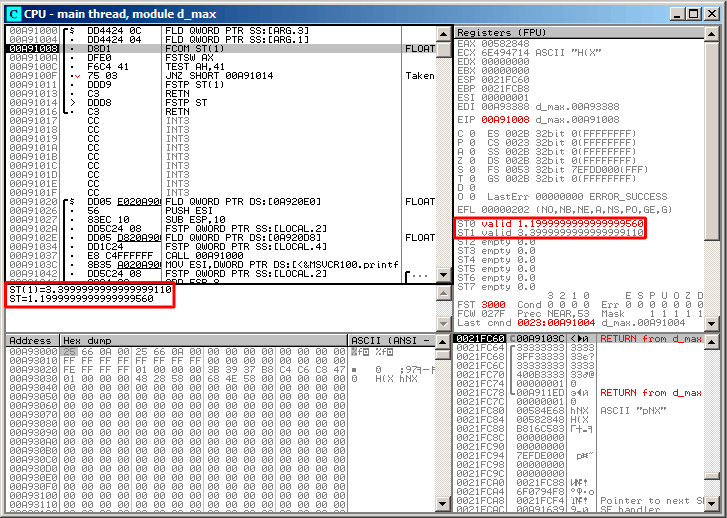
\includegraphics[scale=\FigScale]{patterns/12_FPU/3_comparison/x86/MSVC_Ox/olly1_1.png}
\caption{\olly: \RU{обе \FLD исполнились}\EN{both \FLD are executed}}
\label{fig:FPU_comparison_Ox_case1_olly1}
\end{figure}

\RU{Сейчас будет исполняться }\FCOM\EN{ being executed}: 
\olly \RU{показывает содержимое}\EN{shows the contents of} \ST{0} \AndENRU \ST{1} \RU{для удобства}%
\EN{for convenience}.

\clearpage
\FCOM \RU{сработала}\EN{is done}:

\begin{figure}[H]
\centering
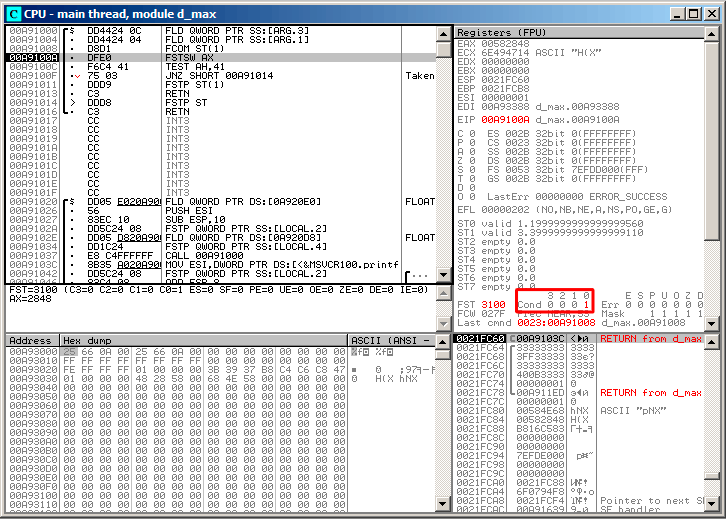
\includegraphics[scale=\FigScale]{patterns/12_FPU/3_comparison/x86/MSVC_Ox/olly1_2.png}
\caption{\olly: \FCOM \RU{исполнилась}\EN{is done}}
\label{fig:FPU_comparison_Ox_case1_olly2}
\end{figure}

\Czero \RU{установлен, остальные флаги сброшены}\EN{is set, all other condition flags are cleared}.

\clearpage
\FNSTSW \RU{сработала}\EN{is done}, \GTT{AX}=0x3100:

\begin{figure}[H]
\centering
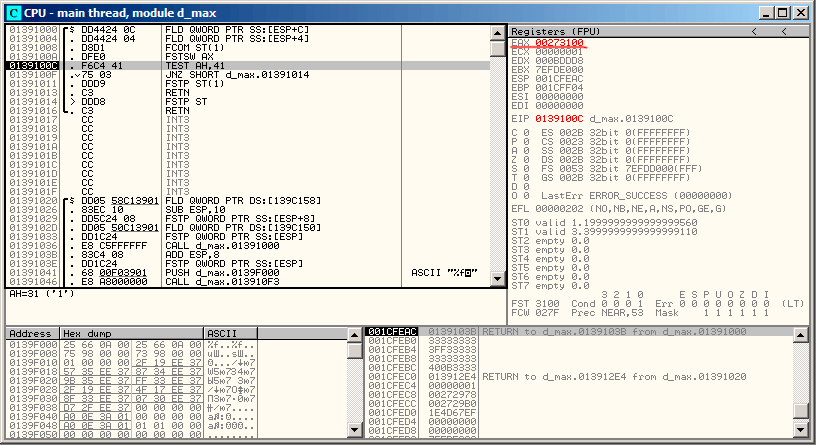
\includegraphics[scale=\FigScale]{patterns/12_FPU/3_comparison/x86/MSVC_Ox/olly1_3.png}
\caption{\olly: \FNSTSW \RU{исполнилась}\EN{is executed}}
\label{fig:FPU_comparison_Ox_case1_olly3}
\end{figure}

\clearpage
\TEST \RU{сработала}\EN{is executed}:

\begin{figure}[H]
\centering
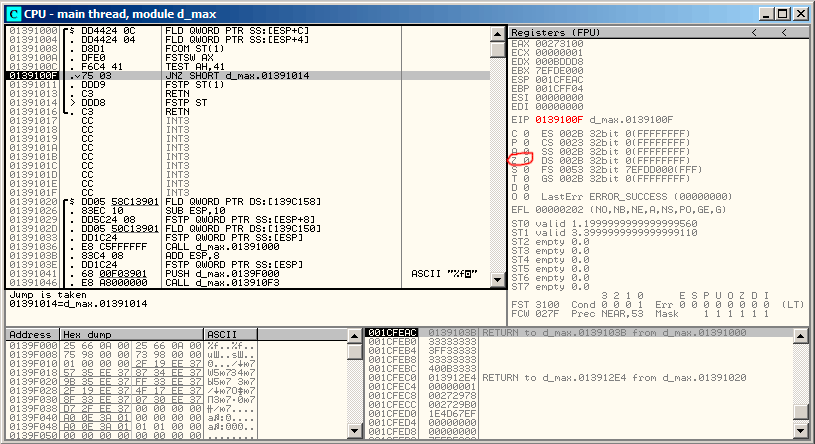
\includegraphics[scale=\FigScale]{patterns/12_FPU/3_comparison/x86/MSVC_Ox/olly1_4.png}
\caption{\olly: \TEST \RU{исполнилась}\EN{is executed}}
\label{fig:FPU_comparison_Ox_case1_olly4}
\end{figure}

ZF=0, \RU{переход сейчас произойдет}\EN{conditional jump is about to trigger now}.

\clearpage
\INS{FSTP ST} (\OrENRU \FSTP \ST{0}) \RU{сработала}\EN{was executed}~---%
\RU{ 1,2 было вытолкнуто из стека, и на вершине осталось 3,4}%
\EN{1.2 was popped from the stack, and 3.4 was left on top}:

\begin{figure}[H]
\centering
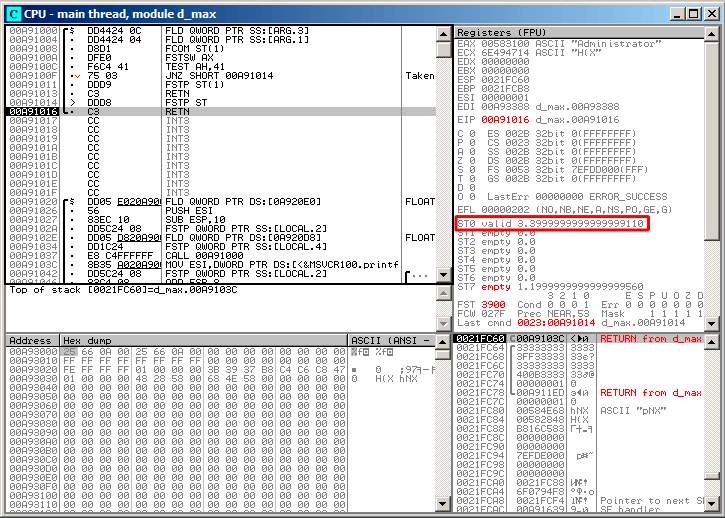
\includegraphics[scale=\FigScale]{patterns/12_FPU/3_comparison/x86/MSVC_Ox/olly1_5.png}
\caption{\olly: \FSTP \RU{исполнилась}\EN{is executed}}
\label{fig:FPU_comparison_Ox_case1_olly5}
\end{figure}

\RU{Видно, что инструкция}\EN{We see that the} \INS{FSTP ST} 
\RU{работает просто как выталкивание одного значения из FPU-стека.}
\EN{instruction works just like popping one value from the FPU stack.}

\clearpage
\myparagraph{\RU{Второй пример с \olly: a=5,6 и b=-4}\EN{Second \olly example: a=5.6 and b=-4}}

\RU{Обе}\EN{Both} \FLD \RU{отработали}\EN{are executed}:

\begin{figure}[H]
\centering
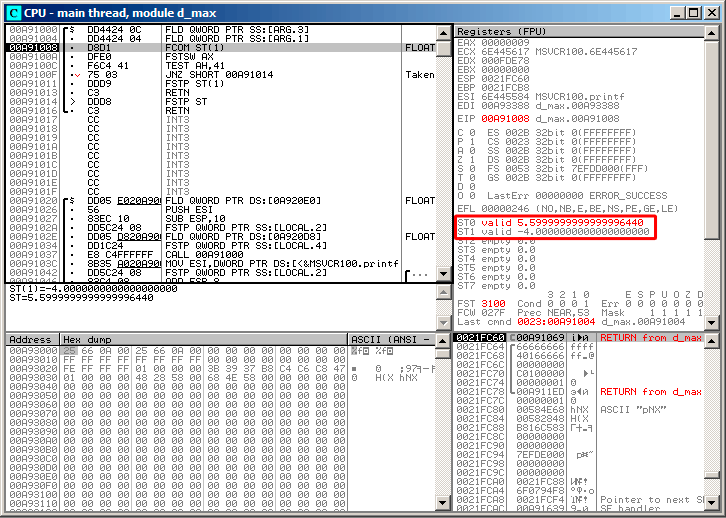
\includegraphics[scale=\FigScale]{patterns/12_FPU/3_comparison/x86/MSVC_Ox/olly2_1.png}
\caption{\olly: \RU{обе \FLD исполнились}\EN{both \FLD are executed}}
\label{fig:FPU_comparison_Ox_case2_olly1}
\end{figure}

\RU{Сейчас будет исполняться \FCOM.}
\EN{\FCOM is about to execute.}

\clearpage
\FCOM \RU{сработала}\EN{is done}:

\begin{figure}[H]
\centering
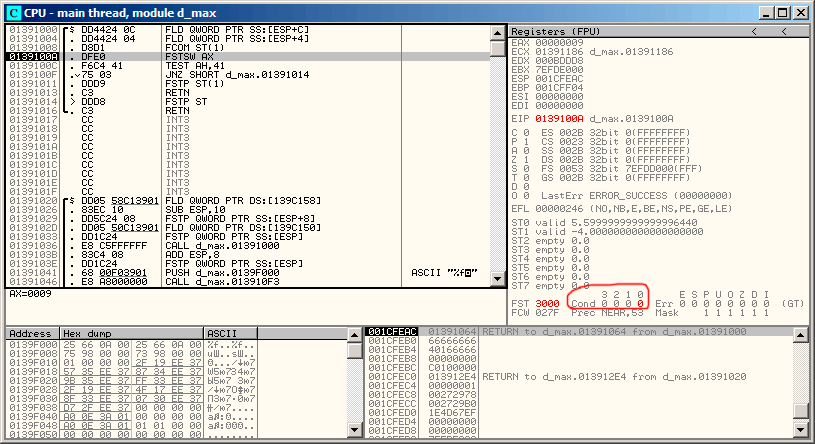
\includegraphics[scale=\FigScale]{patterns/12_FPU/3_comparison/x86/MSVC_Ox/olly2_2.png}
\caption{\olly: \FCOM \RU{исполнилась}\EN{is finished}}
\label{fig:FPU_comparison_Ox_case2_olly2}
\end{figure}

\RU{Все condition-флаги сброшены}\EN{All conditional flags are cleared}.

\clearpage
\FNSTSW \RU{сработала}\EN{done}, \GTT{AX}=0x3000:

\begin{figure}[H]
\centering
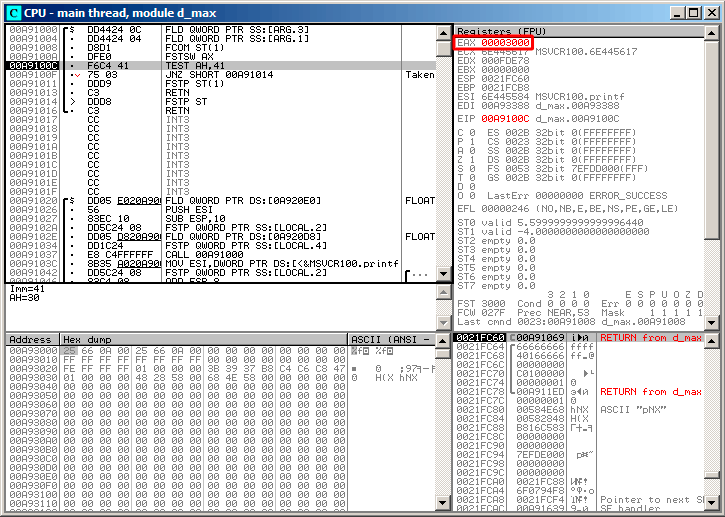
\includegraphics[scale=\FigScale]{patterns/12_FPU/3_comparison/x86/MSVC_Ox/olly2_3.png}
\caption{\olly: \FNSTSW \RU{исполнилась}\EN{was executed}}
\label{fig:FPU_comparison_Ox_case2_olly3}
\end{figure}

\clearpage
\TEST \RU{сработала}\EN{is done}:

\begin{figure}[H]
\centering
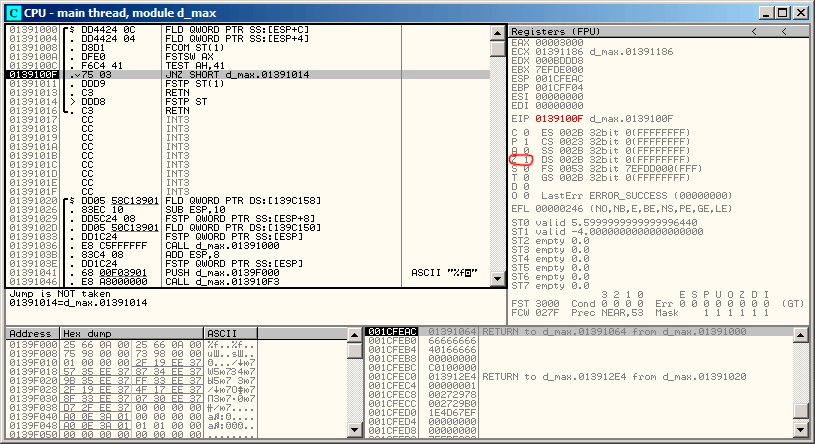
\includegraphics[scale=\FigScale]{patterns/12_FPU/3_comparison/x86/MSVC_Ox/olly2_4.png}
\caption{\olly: \TEST \RU{исполнилась}\EN{was executed}}
\label{fig:FPU_comparison_Ox_case2_olly4}
\end{figure}

ZF=1, \RU{переход сейчас не произойдет}\EN{jump will not happen now}.

\clearpage
\FSTP \ST{1} \RU{сработала: на вершине FPU-стека осталось значение 5,6}\EN{was executed: a value
of 5.6 is now at the top of the FPU stack}.

\begin{figure}[H]
\centering
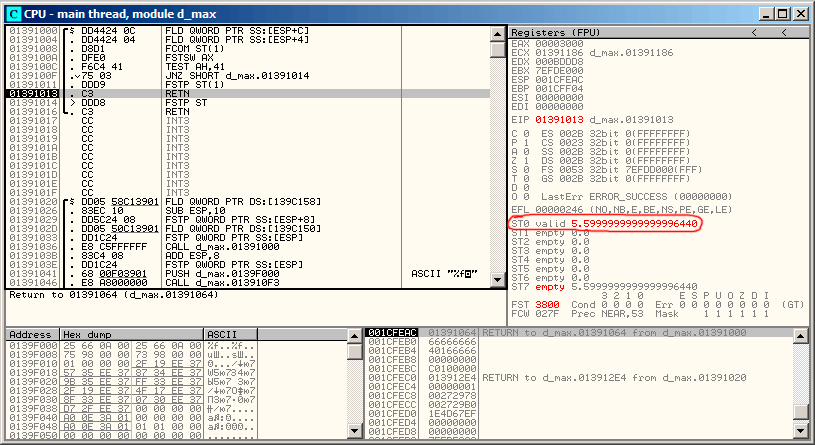
\includegraphics[scale=\FigScale]{patterns/12_FPU/3_comparison/x86/MSVC_Ox/olly2_5.png}
\caption{\olly: \FSTP \RU{исполнилась}\EN{was executed}}
\label{fig:FPU_comparison_Ox_case2_olly5}
\end{figure}

\RU{Видно, что инструкция}\EN{We now see that the} \FSTP \ST{1} 
\RU{работает так: оставляет значение на вершине стека, но обнуляет регистр \ST{1}.}
\EN{instruction works as follows: it leaves what was at the top of the stack, but clears \ST{1}.}

\fi
